\documentclass[11pt]{article}

\usepackage[colorlinks=true]{hyperref}

% This is a toggle for whether the solutions should be included in output of this document
\newif\ifSolutions
%\Solutionsfalse  % this is used to exclude the solutions
\Solutionstrue  % this is used to include the solutions


\usepackage[left=0.8in, right=0.8in, top=0.7in, bottom=1in, includefoot]{geometry}
\usepackage{fancyhdr}
\usepackage{array}
\usepackage{multicol}
\setlength{\parindent}{0mm}
\setlength{\parskip}{5pt}
\usepackage{sectsty}
\allsectionsfont{\sffamily}
\setlength{\headheight}{2cm}
\usepackage{amsmath,amssymb,bm}
\usepackage{booktabs}
\usepackage{graphicx}
\usepackage{color}
\usepackage{cancel}
\usepackage{comment}
\usepackage{hyperref}
\usepackage{subfig}
\usepackage{multirow}
\usepackage{placeins}

% Global definitions
%
% boldface letters
%
%\newcommand{\boldface}[1]{\mathbf{#1}}   % upright
\newcommand{\boldface}[1]{\boldsymbol{#1}}  % italic (slanted)
%
\newcommand{\bfa}{\boldface{a}}
\newcommand{\bfb}{\boldface{b}}
\newcommand{\bfc}{\boldface{c}}
\newcommand{\bfd}{\boldface{d}}
\newcommand{\bfe}{\boldface{e}}
\newcommand{\bff}{\boldface{f}}
\newcommand{\bfg}{\boldface{g}}
\newcommand{\bfh}{\boldface{h}}
\newcommand{\bfi}{\boldface{i}}
\newcommand{\bfj}{\boldface{j}}
\newcommand{\bfk}{\boldface{k}}
\newcommand{\bfl}{\boldface{l}}
\newcommand{\bfm}{\boldface{m}}
\newcommand{\bfn}{\boldface{n}}
\newcommand{\bfo}{\boldface{o}}
\newcommand{\bfp}{\boldface{p}}
\newcommand{\bfq}{\boldface{q}}
\newcommand{\bfr}{\boldface{r}}
\newcommand{\bfs}{\boldface{s}}
\newcommand{\bft}{\boldface{t}}
\newcommand{\bfu}{\boldface{u}}
\newcommand{\bfv}{\boldface{v}}
\newcommand{\bfw}{\boldface{w}}
\newcommand{\bfx}{\boldface{x}}
\newcommand{\bfy}{\boldface{y}}
\newcommand{\bfz}{\boldface{z}}
%
\newcommand{\bfA}{\boldface{A}}
\newcommand{\bfB}{\boldface{B}}
\newcommand{\bfC}{\boldface{C}}
\newcommand{\bfD}{\boldface{D}}
\newcommand{\bfE}{\boldface{E}}
\newcommand{\bfF}{\boldface{F}}
\newcommand{\bfG}{\boldface{G}}
\newcommand{\bfH}{\boldface{H}}
\newcommand{\bfI}{\boldface{I}}
\newcommand{\bfJ}{\boldface{J}}
\newcommand{\bfK}{\boldface{K}}
\newcommand{\bfL}{\boldface{L}}
\newcommand{\bfM}{\boldface{M}}
\newcommand{\bfN}{\boldface{N}}
\newcommand{\bfO}{\boldface{O}}
\newcommand{\bfP}{\boldface{P}}
\newcommand{\bfQ}{\boldface{Q}}
\newcommand{\bfR}{\boldface{R}}
\newcommand{\bfS}{\boldface{S}}
\newcommand{\bfT}{\boldface{T}}
\newcommand{\bfU}{\boldface{U}}
\newcommand{\bfV}{\boldface{V}}
\newcommand{\bfW}{\boldface{W}}
\newcommand{\bfX}{\boldface{X}}
\newcommand{\bfY}{\boldface{Y}}
\newcommand{\bfZ}{\boldface{Z}}

\newcommand{\bfFe}{\boldface{F}_{\text{e}}}
\newcommand{\bfFp}{\boldface{F}_{\text{p}}}
\newcommand{\bfepse}{\pmb{\varepsilon}_{\text{e}}}
\newcommand{\bfepsp}{\pmb{\varepsilon}_{\text{p}}}
\newcommand{\bfeps}{\pmb{\varepsilon}}

%
% boldface greek symbols
%
\newcommand{\bfalpha}{\boldsymbol{\alpha}}
\newcommand{\bfbeta}{\boldsymbol{\beta}}
\newcommand{\bfgamma}{\boldsymbol{\gamma}}
\newcommand{\bfdelta}{\boldsymbol{\delta}}
\newcommand{\bfepsilon}{\pmb{\varepsilon}}
\newcommand{\bfzeta}{\boldsymbol{\zeta}}
\newcommand{\bfeta}{\boldsymbol{\eta}}
\newcommand{\bftheta}{\boldsymbol{\theta}}
\newcommand{\bfkappa}{\boldsymbol{\kappa}}
\newcommand{\bflambda}{\boldsymbol{\lambda}}
\newcommand{\bfrho}{\boldsymbol{\rho}}
\newcommand{\bfmu}{\boldsymbol{\mu}}
\newcommand{\bfnu}{\boldsymbol{\nu}}
\newcommand{\bfpi}{\boldsymbol{\pi}}
\newcommand{\bfxi}{\boldsymbol{\xi}}
\newcommand{\bfsigma}{\boldsymbol{\sigma}}
\newcommand{\bftau}{\boldsymbol{\tau}}
\newcommand{\bfphi}{\boldsymbol{\phi}}
\newcommand{\bfvarphi}{\boldsymbol{\varphi}}
\newcommand{\bfchi}{\boldsymbol{\chi}}
\newcommand{\bfomega}{\boldsymbol{\omega}}
\newcommand{\bfnull}{\boldsymbol{0}}
%
\newcommand{\bfGamma}{\boldsymbol{\Gamma}}
\newcommand{\bfDelta}{\boldsymbol{\Delta}}
\newcommand{\bfTheta}{\boldsymbol{\Theta}}
\newcommand{\bfLambda}{\boldsymbol{\Lambda}}
\newcommand{\bfPi}{\boldsymbol{\Pi}}
\newcommand{\bfXi}{\boldsymbol{\Xi}}
\newcommand{\bfSigma}{\boldsymbol{\Sigma}}
\newcommand{\bfPhi}{\boldsymbol{\Phi}}
\newcommand{\bfChi}{\boldsymbol{\Chi}}
\newcommand{\bfOmega}{\boldsymbol{\Omega}}
\newcommand{\bfnabla}{\boldsymbol{\nabla}}
\newcommand{\laplace}{\boldsymbol{\Delta}}
%
% caligraphic letters
%
\newcommand{\calA}{\mathcal{A}}
\newcommand{\calB}{\mathcal{B}}
\newcommand{\calC}{\mathcal{C}}
\newcommand{\calD}{\mathcal{D}}
\newcommand{\calE}{\mathcal{E}}
\newcommand{\calF}{\mathcal{F}}
\newcommand{\calG}{\mathcal{G}}
\newcommand{\calH}{\mathcal{H}}
\newcommand{\calI}{\mathcal{I}}
\newcommand{\calJ}{\mathcal{J}}
\newcommand{\calK}{\mathcal{K}}
\newcommand{\calL}{\mathcal{L}}
\newcommand{\calM}{\mathcal{M}}
\newcommand{\calN}{\mathcal{N}}
\newcommand{\calO}{\mathcal{O}}
\newcommand{\calP}{\mathcal{P}}
\newcommand{\calQ}{\mathcal{Q}}
\newcommand{\calR}{\mathbb{R}}
\newcommand{\calS}{\mathcal{S}}
\newcommand{\calT}{\mathcal{T}}
\newcommand{\calU}{\mathcal{U}}
\newcommand{\calV}{\mathcal{V}}
\newcommand{\calW}{\mathcal{W}}
\newcommand{\calX}{\mathcal{X}}
\newcommand{\calY}{\mathcal{Y}}
\newcommand{\calZ}{\mathcal{Z}}
% .. define more if needed
%
% double stroke
%
\newcommand{\dsA}{\mathbb{A}}
\newcommand{\dsB}{\mathbb{B}}
\newcommand{\dsC}{\mathbb{C}}
\newcommand{\dsD}{\mathbb{D}}
\newcommand{\dsE}{\mathbb{E}}
\newcommand{\dsF}{\mathbb{F}}
\newcommand{\dsG}{\mathbb{G}}
\newcommand{\dsH}{\mathbb{H}}
\newcommand{\dsI}{\mathbb{I}}
\newcommand{\dsJ}{\mathbb{J}}
\newcommand{\dsK}{\mathbb{K}}
\newcommand{\dsL}{\mathbb{L}}
\newcommand{\dsM}{\mathbb{M}}
\newcommand{\dsN}{\mathbb{N}}
\newcommand{\dsO}{\mathbb{O}}
\newcommand{\dsP}{\mathbb{P}}
\newcommand{\dsQ}{\mathbb{Q}}
\newcommand{\dsR}{\mathbb{R}}
\newcommand{\dsS}{\mathbb{S}}
\newcommand{\dsT}{\mathbb{T}}
\newcommand{\dsU}{\mathbb{U}}
\newcommand{\dsV}{\mathbb{V}}
\newcommand{\dsW}{\mathbb{W}}
\newcommand{\dsX}{\mathbb{X}}
\newcommand{\dsY}{\mathbb{Y}}
\newcommand{\dsZ}{\mathbb{Z}}



\newcommand{\vect}[1]{\mathbf{#1}}
\newcommand{\grvect}[1]{\mbox{\boldmath{$#1$}}}
\newcommand{\perm}{\mbox{{\Huge $\epsilon$}}}
\newcommand{\transvect}[1]{\vect{#1}^{\mbox{\footnotesize T}}}
\newcommand{\invvect}[1]{\vect{#1}^{\mbox{\footnotesize -1}}}
\newcommand{\partderiv}[2]{\frac{\partial #1}{\partial #2}}
\newcommand{\partderivv}[2]{\frac{\partial^2 #1}{\partial #2^2}}
\newcommand{\totalderiv}[2]{\frac{d #1}{d #2}}

\newcommand{\mg}[1]{{\boldsymbol{#1}}}
\newcommand{\mf}[1]{{\mathfrak{#1}}}
\newcommand{\mfb}[1]{{\boldsymbol{\mathfrak{#1}}}}
\newcommand{\ms}[1]{{\mathscr{#1}}}
\newcommand{\mb}[1]{{\mathbf{#1}}}
\newcommand{\mbb}[1]{{\mathbb{#1}}}
\newcommand{\mbbu}[1]{{\underline{\mathbb{#1}}}\vphantom{#1}}
\newcommand{\mbu}[1]{{\underline{\mathbf{#1}}}\vphantom{#1}}
\newcommand{\mgu}[1]{{\underline{\boldsymbol{#1}}}\vphantom{#1}}
\newcommand{\mr}[1]{{\mathrm{#1}}}
\newcommand{\msf}[1]{{\mathsf{#1}}}
\newcommand{\msfb}[1]{{\boldsymbol{\mathsf{#1}}}}

\newcommand{\dotprod}{\stackrel{\scriptscriptstyle \bullet}{}}
\newcommand{\half}{\frac{1}{2}}
\newcommand{\T}{^{\mathsf{T}}} % x^{T}
\newcommand{\mT}{^{\mathsf{-T}}} % x^{-T}
\newcommand{\wass}{\mathsf{wass}}
\newcommand{\eff}{\mathsf{eff}}
\newcommand{\me}{^{\mathrm{-1}}} % x^{-1}
\newcommand{\Rset}{\ensuremath{\mathbb{R}}}
\newcommand{\Kset}{\ensuremath{K}}
\newcommand{\bul}{$\bullet\;$}
%\newcommand{\red}{\mathrm{red}}
\newcommand{\Fe}{\mathbf{F}_\mathbf{e}}
\newcommand{\Fp}{\mathbf{F}_\mathbf{p}}
\def\rel{{\mathrm{rel}}}

%\newcommand{\D}{\displaystyle}
\newcommand{\abs}{\rule[-1cm]{0cm}{1cm}}
\newcommand{\babs}{\rule[-1cm]{0cm}{2cm}}

\newlength{\boxwidth}
\setlength{\boxwidth}{\textwidth}
\addtolength{\boxwidth}{-1cm}

\newcommand\pl{\partial}
\def\dd{\;\!\mathrm{d}}
\def\DD{\;\!\mathrm{D}}
\def\Lin{\R^{d\times d}} 
\def\R{I\!R}
\def\AM{{\mathrm{AM}}}

\def\btheorem{\begin{theorem}}
\def\etheorem{\end{theorem}}
\def\blemma{\begin{lemma}}
\def\elemma{\end{lemma}}
\def\bproposition{\begin{proposition}}
\def\eproposition{\end{proposition}}
\def\bcorollary{\begin{corollary}}
\def\ecorollary{\end{corollary}}
\def\bdefinition{\begin{definition}}
\def\edefinition{\end{definition}}
\def\bexample{\begin{example}}
\def\eexample{\end{example}}
\def\bremark{\begin{remark}}
\def\eremark{\end{remark}}
\def\bproblem#1{\medskip \noindent {\bf #1}\sl \\ }
\def\eproblem{\rm \medskip}
\newcommand{\bma}{ \left( \ba}
\newcommand{\ema}{ \ea \right)}
\newcommand{\set}[2]{\big\{\: #1 \: \big| \: #2 \:\big\} }
\def\cD{\mathcal{D}}
\def\cL{\mathcal{L}}
\def\cG{\mathcal{G}}
\def\cI{\mathcal{I}}
\def\cJ{\mathcal{J}}
\def\ccA{\mathcal{A}}
\def\rmD{\mathrm{D}}
\def\bbQ{\mathbb{Q}}
\def\bbA{\fg{A\!\!\!A}}
\def\fg{\boldsymbol}
\def\mdot{\fg{:}}
\def\vdot{\fg{\cdot}}
\newcommand{\el}{\mathsf{el}}
\def\id{{\bfI}}
\def\eqldef{{\:{\stackrel{\mathrm{def}}{=}}\:}}
\newcommand{\eps}{\varepsilon}
\def\ol{\overline}
\def\wt{\widetilde}
\def\wh{\widehat}
\def\ds{\displaystyle}
\def\ts{\textstyle}
\def\mtr{^\mathrm{-T}}
\def\inh{^\mathrm{inh}}
\DeclareMathOperator{\divv}{div}
\DeclareMathOperator{\grad}{grad}
\DeclareMathOperator{\tr}{tr}
\DeclareMathOperator{\curl}{curl}
\DeclareMathOperator{\Curl}{Curl}
%\DeclareMathOperator{\T}{T}
\DeclareMathOperator{\argmin}{{arg\,min}}
\DeclareMathOperator{\diag}{diag}
\DeclareMathOperator{\trace}{tr}
\DeclareMathOperator{\sign}{sign}
\DeclareMathOperator{\dev}{dev}
\DeclareMathOperator{\cof}{cof}
\DeclareMathOperator{\sym}{sym}
\DeclareMathOperator{\skews}{skw}
\def\Felast{\bfF_\mathbf{\!e}}
\def\Fplast{\bfF_\mathbf{\!p}}
\def\Cplast{\bfC_\mathbf{\!p}}
\def\epselast{\bfeps_\mathbf{\!e}}
\def\epsplast{\bfeps_\mathbf{\!p}}
\def\GLin{\mbox{{\sf GL}$(d)$}}  %{\R^{d\times d}_*}% invertible matrices
\def\Lin{\R^{d\times d}}        % all d times d matrices
\def\reff#1{(\ref{#1})}
\def\red{{\mathrm{red}}}
\def\rep{{\mathrm{rep}}}
\def\cond{{\mathrm{cond}}}
\newcommand{\kopfcolor}{\color{red}}
\newcommand{\er}{\hspace*{4cm}}
\newcommand{\n}{{\rm n}}
\newcommand{\nn}{{\rm n+1}}
\newcommand{\PsiS}{\Psi_\mathrm{S}}
\newcommand{\PsiV}{\Psi_\mathrm{V}}
\newcommand{\PsiI}{\Psi_\mathrm{I}}
\newcommand{\cA}{c_\mathrm{A}}
\newcommand{\cM}{c_\mathrm{M}}

\newcommand{\calAe}{\underset{e=1}{\overset{n_e}{\mathcal{A}}}}
\newcommand{\Grad}{\text{Grad}}
\newcommand{\tcr}{\tau_{\text{crit}}}
\newcommand{\be}{\begin{equation}\nonumber}
\newcommand{\ee}{\end{equation}}
\newcommand{\beq}{\begin{eqnarray}}
\newcommand{\eeq}{\end{eqnarray}}
\newcommand{\bem}{\begin{multline}}
\newcommand{\eem}{\end{multline}}
\newcommand{\ba}{\begin{align}}
\newcommand{\ea}{\end{align}}
\newcommand{\bfzero}{{\fg0}}

\renewcommand{\figurename}{Figure}
\renewcommand{\tablename}{Table}

\newcommand{\fp}[2]{\frac{\partial #1}{\partial #2} }
\newcommand{\LR}{{\qquad \Leftrightarrow \qquad }}
\newcounter{problem}
\newcounter{points}
\newcounter{stretchPoints}

\newcommand{\head}[3]{

\begin{center}
\section*{Homework Set \##1 \ifSolutions Solutions \fi}
assigned: #2\\
due: #3, 11:00 pm\\
in your repo at /cs/cs181j/2015/fall/students/your\_user\_name/cs181j \\
\end{center}
\hrule
\vskip 0.1cm
}

\newcommand{\prob}[1]{\par\vskip 0.5cm \stepcounter{problem}\subsubsection*{Problem \arabic{problem} \ \small (#1 points).}\addtocounter{points}{#1}}
\newcommand{\total}{
\begin{flushright}
\small\par\vskip 0.3cm \textit{total: \arabic{points} points ({\color{blue}+\arabic{stretchPoints} stretch points})}
\end{flushright}
}

\newcommand{\eprob}[2]{\par\vskip 0.5cm \stepcounter{problem}\subsubsection*{Problem \arabic{problem}: #2 \ \small (#1 points).}\addtocounter{points}{#1}}

\newcommand{\estretchprob}[3]{\par\vskip 0.5cm \stepcounter{problem}\subsubsection*{Problem \arabic{problem}: #3 \ \small (#1 points ({\color{blue}+#2 stretch points}) ).}\addtocounter{points}{#1}\addtocounter{stretchPoints}{#2}}


%\endinput

\usepackage{afterpage}
\usepackage{enumerate}

\begin{document}
\sffamily
\pagestyle{fancy}
\renewcommand{\headrulewidth}{0.4pt}
\fancyfoot[C]{\sffamily \thepage{}}
\fancyhead[C]{\vskip 0.7cm \sffamily\footnotesize \textbf{cs181j -- High Performance Computing} \hfill \name\\ Fall 2015 \hfill Harvey Mudd College}

% Convenience function used for including a figure
\newcommand\Figure[3]
{
    \begin{figure}[h!]
        \begin{center}
    \includegraphics[width=#3 in]{#1}
    \caption{\label{fig:#1} {#2}}
    \end{center}
    \end{figure}
}

\newcommand\TwoFigure[7]
{
    \begin{figure}[h!]
        \subfloat[#2]{\includegraphics[width=#7 in]{#1}}
    \hfill
        \subfloat[#4]{\includegraphics[width=#7 in]{#3}}
        \caption{\label{fig:#6}#5}
    \end{figure}
}

\newcommand\TwoFigureVertical[7]
{
    \begin{figure}[h!]
        \subfloat[#2]{\includegraphics[width=#7 in]{#1}}

        \subfloat[#4]{\includegraphics[width=#7 in]{#3}}
        \caption{\label{fig:#6}#5}
    \end{figure}
}


\fancyhead[RL]{}

%\newcommand{\name}{I forgot to change my name}


\head{8}{Friday, November 6, 2015}{Wednesday, November 11, 2015}

In this homework assignment, you're going to thread several problems with \href{https://www.threadingbuildingblocks.org/}{threading building blocks}.  As usual, I have provided serial versions of the algorithms as well as all the testing, timing, and rendering bits.  You should only have to insert code in the \texttt{TODOs}.

Note: there is a compilable, runnable, and rather boring \texttt{Main0.cc} that contains much if not all of the syntax you'll need for the assignment.


\eprob{10}{FindIndexOfNearestPoint redux, now with tbb for added freshness}

Our first example will be a warm-up; you'll revisit the \texttt{FindIndexOfNearestPoint} algorithm.  Write the \texttt{findIndexOfClosestPoint\_tbb} function in \texttt{FindIndexOfNearestPoint\_functions.h}.  The performance plots are included here; how does tbb compare against openmp from your last assignment (automatically included here)?

\ifSolutions
\textbf{Solution:}
{
  \begin{figure}[ht]
    \begin{center}
    \begin{tabular}{cc}
    \subfloat[omp log]{
\includegraphics[width=3.0in, trim=1.1in .5in .75in .5in, clip]{../hw7/figures/FindIndexOfClosestPoint_threadedVersusSerial_log_shuffler}} &
    \subfloat[omp linear]{
\includegraphics[width=3.0in, trim=1.1in .5in .75in .5in, clip]{../hw7/figures/FindIndexOfClosestPoint_threadedVersusSerial_linear_shuffler}} \\
    \subfloat[tbb log]{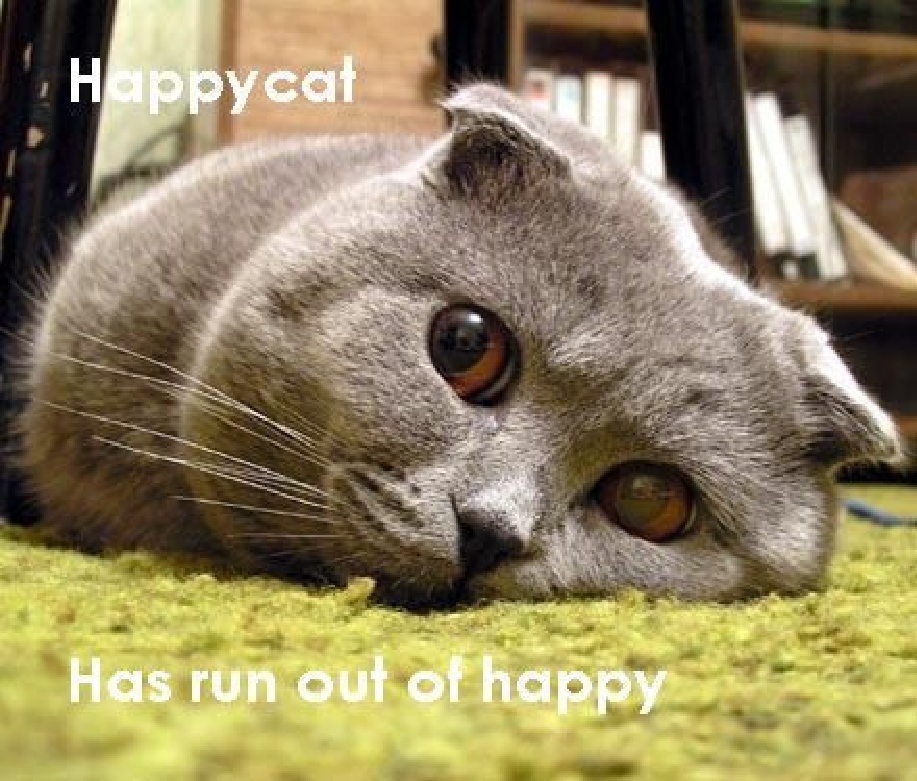
\includegraphics[width=3.0in, trim=1.1in .5in .75in .5in, clip]{figures/FindIndexOfClosestPoint_tbbVersusSerial_log_shuffler}} &
    \subfloat[tbb linear]{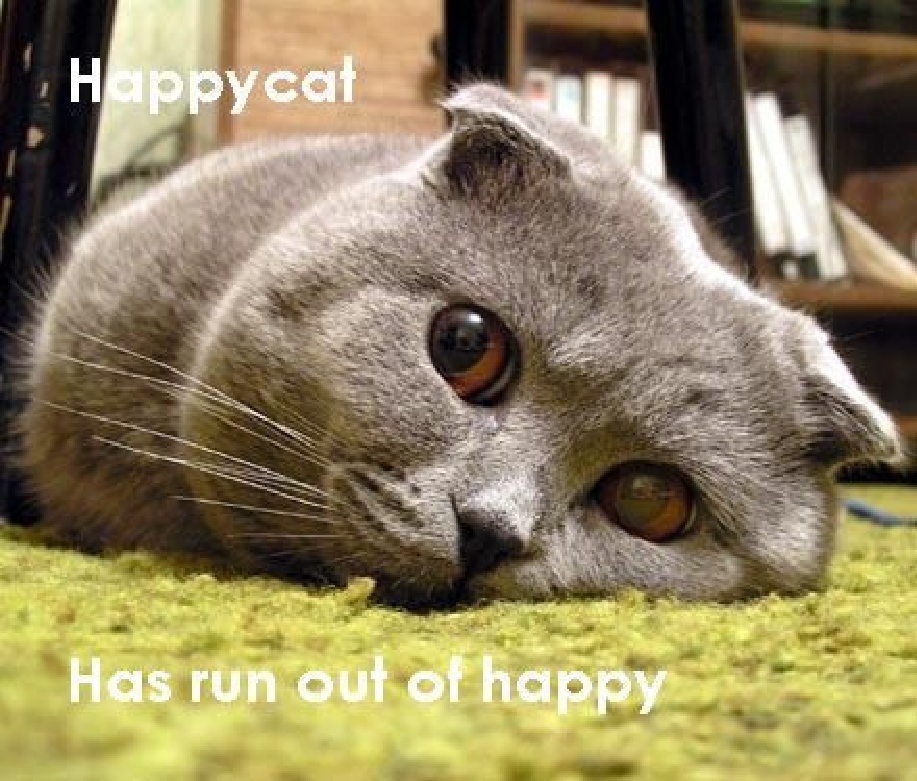
\includegraphics[width=3.0in, trim=1.1in .5in .75in .5in, clip]{figures/FindIndexOfClosestPoint_tbbVersusSerial_linear_shuffler}} \\
    \subfloat[speedup of omp over tbb]{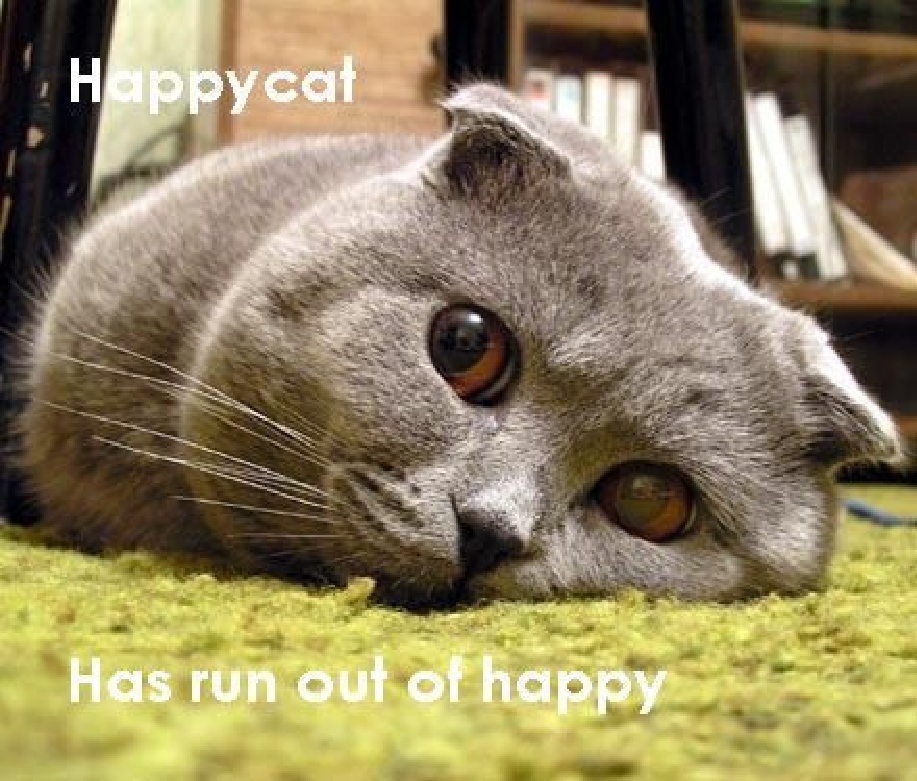
\includegraphics[width=3.0in, trim=1.1in .5in .75in .5in, clip]{figures/FindIndexOfClosestPoint_ompVersusTbb_shuffler}} &
    \subfloat[speedup of tbb over omp]{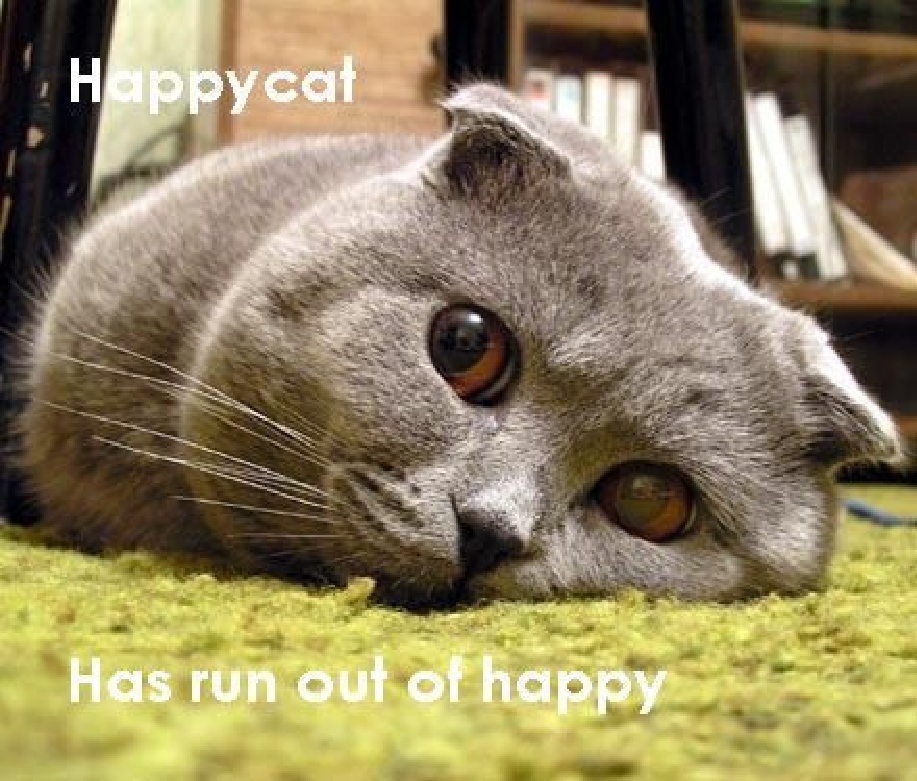
\includegraphics[width=3.0in, trim=1.1in .5in .75in .5in, clip]{figures/FindIndexOfClosestPoint_tbbVersusOmp_shuffler}} \\
    \end{tabular}
    \end{center}
    \caption{Performance for FindIndexOfNearestPoint}
    \label{fig:FindIndexOfNearestPoint}
  \end{figure}
}


\FloatBarrier

\vfill






\eprob{20}{TLB with TBB (brought to you by TLC)}

We will use the example of calculating the sum of polynomials to explore the issue of \textbf{T}hread \textbf{L}oad \textbf{B}alancing for different threading systems.

\[\displaystyle\sum_i c_0 + c_1 \text{input}[i] + c_2 \text{input}[i]^2 + c_3 \text{input}[i]^3 + ...\]

You will make two implementations, using \texttt{openmp}  and \texttt{tbb}. For a fixed \texttt{maxPolynomialOrder}, we'll explore performance versus input size and total number of threads used. You'll run these calculations in one of two ``modes'': \texttt{Fixed} or \texttt{ProportionalToIndex}.  

In \texttt{Fixed} mode, each input will be evaluated up to the same polynomial order, \texttt{maxPolynomialOrder}.  This is the easiest case for threading systems to balance the load because all the tasks take around the same time.

In \texttt{ProportionalToIndex} mode, each input will be evaluated up to a polynomial order proportional to that input's index.  That is, input $4567$ of $100000$ inputs with a \texttt{maxPolynomialOrder} of $50$ will only compute up to a polynomial order of $4567/100000*50 = 2$, and input number $87654$ will compute up to a polynomial order of $43$.  This second version will induce some load imbalance to the problem.

Note: I have provided data for \texttt{std::thread}, but I'm not making you do it (because it's boring and slow).

\begin{enumerate}[a)]
\item Implement the \texttt{openmp} version of the polynomial sum calculator in \texttt{calculateSumOfPolynomials\_omp}.  
In order to support different scheduling policies (static, dynamic, guided), I use the \texttt{omp\_set\_schedule} method in \texttt{Main2.cc}.  
\textbf{The only trick is that you have to add the clause \texttt{schedule(runtime)} to your \texttt{pragma omp} line} in \texttt{calculateSumOfPolynomials\_omp}.

You don't need to say anything for this part of the problem, the plot will come later.

\item Implement the \texttt{tbb} version of the polynomial sum calculator in \texttt{calculateSumOfPolynomials\_tbb}.  

You don't need to say anything for this part of the problem, the plot will come later.

\item Use the provided rendering script to make speedup plots versus input size and number of threads for \texttt{Fixed} and \texttt{ProportionalToIndex} modes for all versions.  You shouldn't have to modify the script at all.
The script also makes 2d line plots of the speedup of the five threading methods for the largest, smallest, and a middle input size.  
All plots are already included below.  Comment on your results. What are the strengths and weaknesses of each threading system?
\end{enumerate}

\ifSolutions
\textbf{Solution:}

{
  \begin{figure}[ht]
    \begin{center}
    \begin{tabular}{cc}
    \subfloat[omp static]{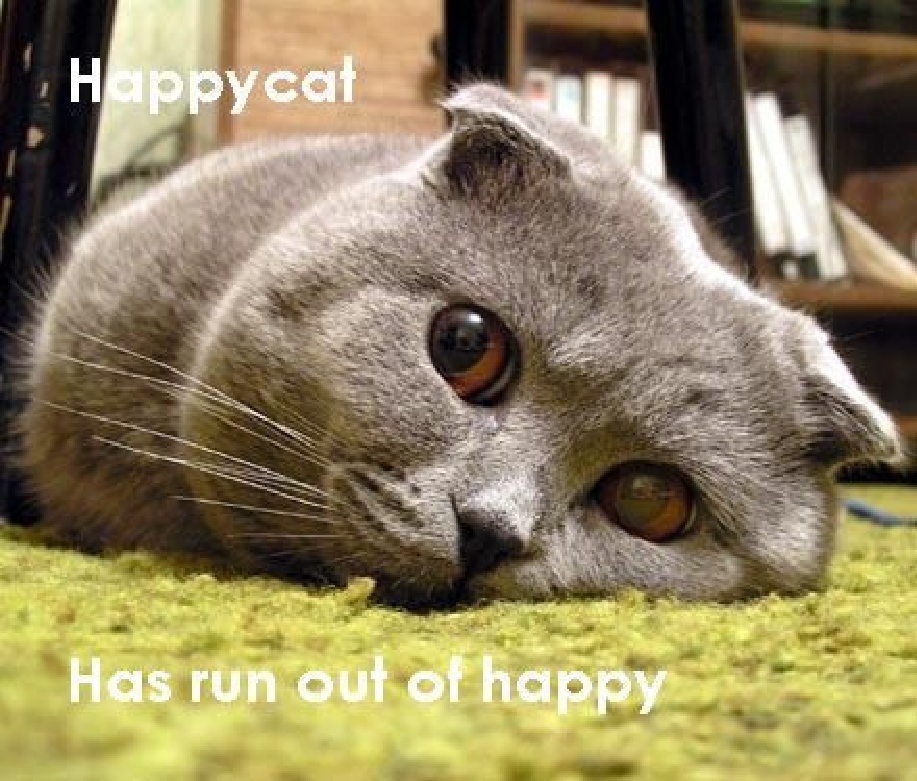
\includegraphics[width=3.25in, trim=1.25in 0.80in 0.90in 0.75in, clip]{figures/Main2_Fixed_ompStatic_shuffler}} &
    \subfloat[std::thread]{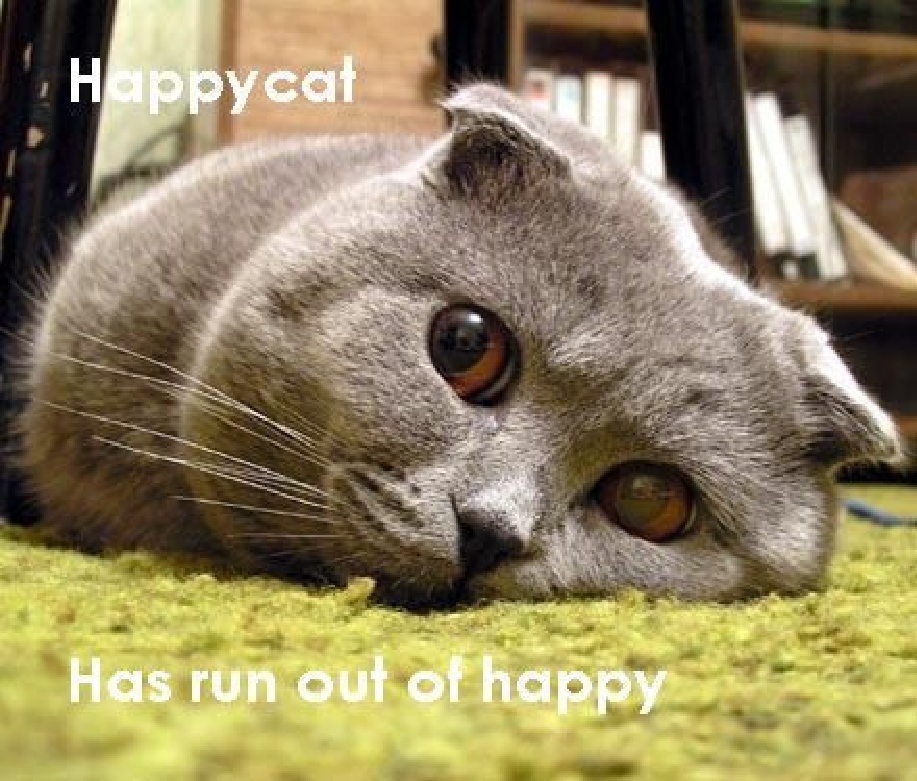
\includegraphics[width=3.25in, trim=1.25in 0.80in 0.90in 0.75in, clip]{figures/Main2_Fixed_stdThread_shuffler}} \\
    \subfloat[omp dynamic]{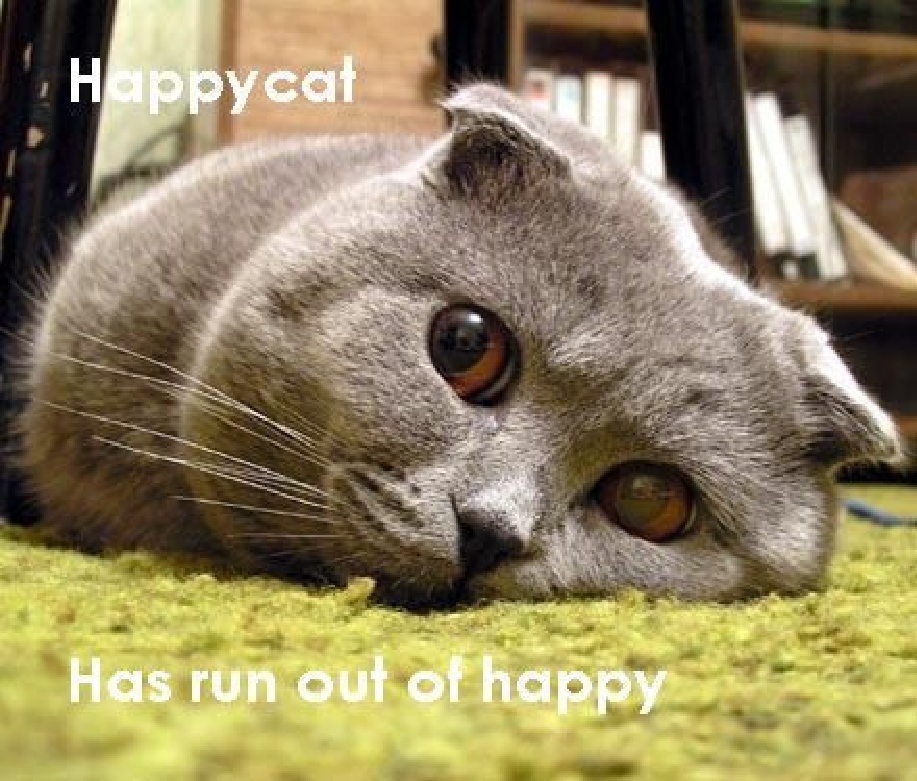
\includegraphics[width=3.25in, trim=1.25in 0.80in 0.90in 0.75in, clip]{figures/Main2_Fixed_ompDynamic_shuffler}} & \\
    \subfloat[omp guided]{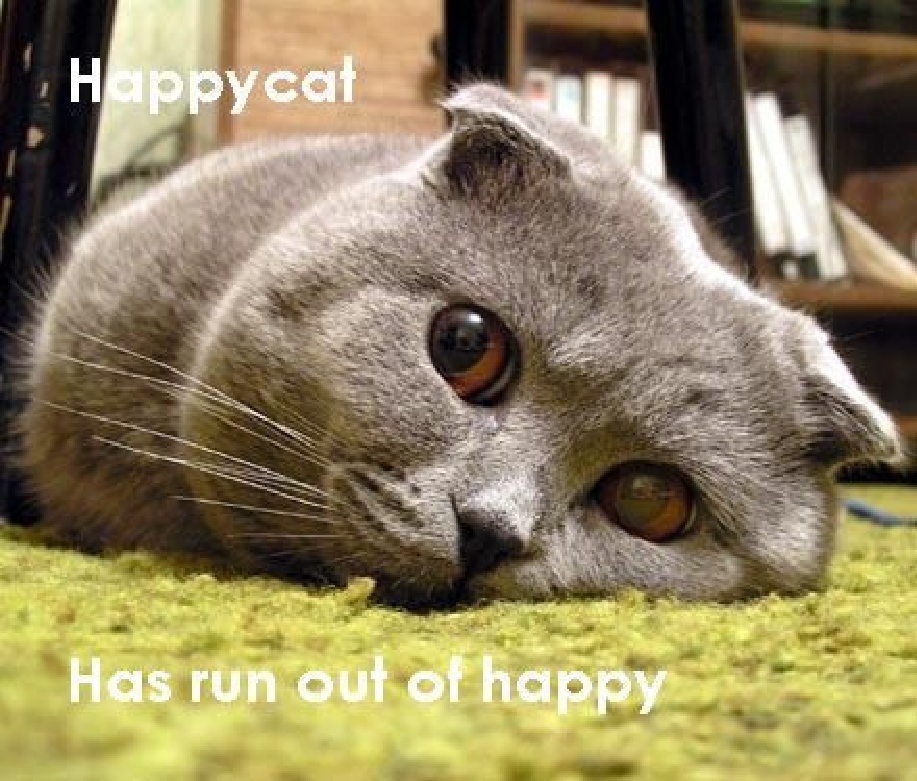
\includegraphics[width=3.25in, trim=1.25in 0.80in 0.90in 0.75in, clip]{figures/Main2_Fixed_ompGuided_shuffler}} &
    \subfloat[tbb]{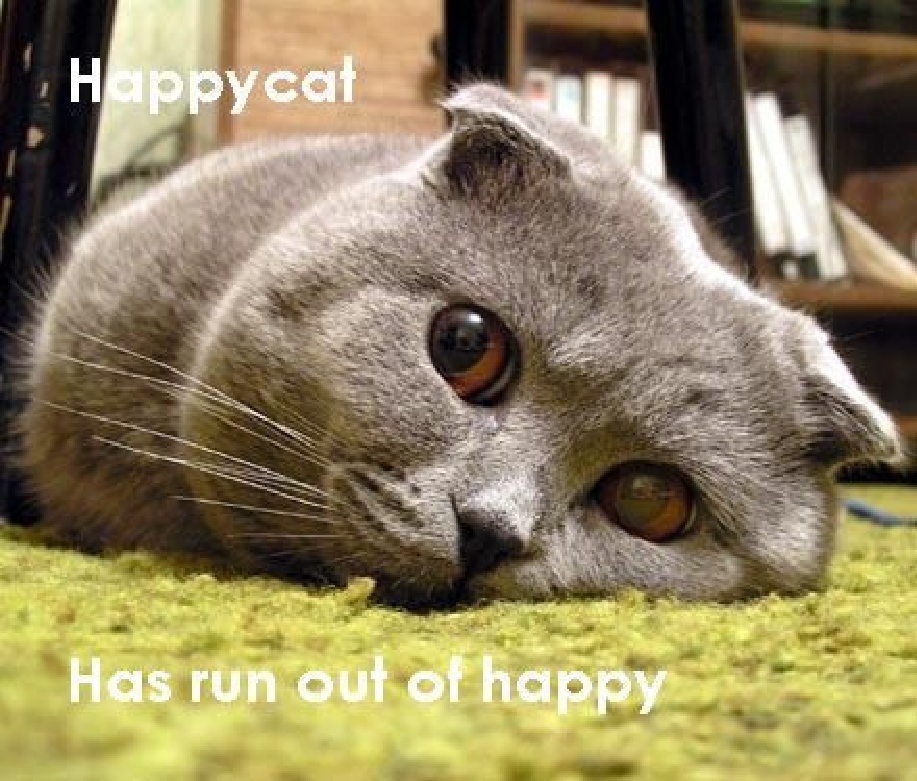
\includegraphics[width=3.25in, trim=1.25in 0.80in 0.90in 0.75in, clip]{figures/Main2_Fixed_tbb_shuffler}} \\
    \end{tabular}
    \end{center}
    \caption{Performance for Fixed polynomial order}
    \label{fig:Main2_fixed}
  \end{figure}
}

{
  \begin{figure}[ht]
    \begin{center}
    \begin{tabular}{cc}
    \subfloat[omp static]{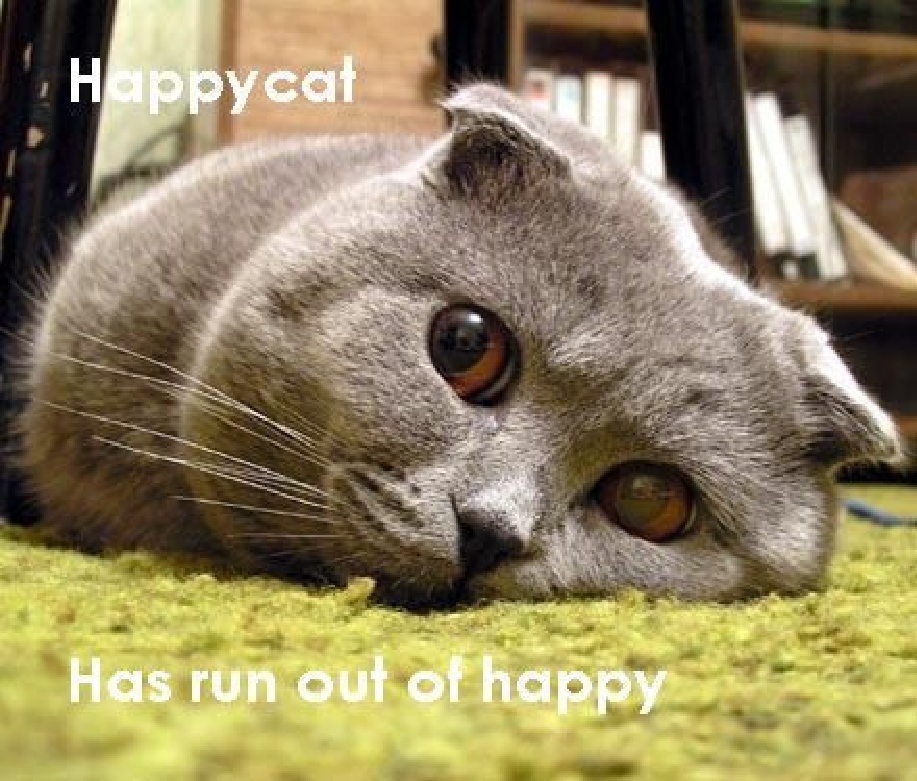
\includegraphics[width=3.25in, trim=1.25in 0.80in 0.90in 0.75in, clip]{figures/Main2_ProportionalToIndex_ompStatic_shuffler}} &
    \subfloat[std::thread]{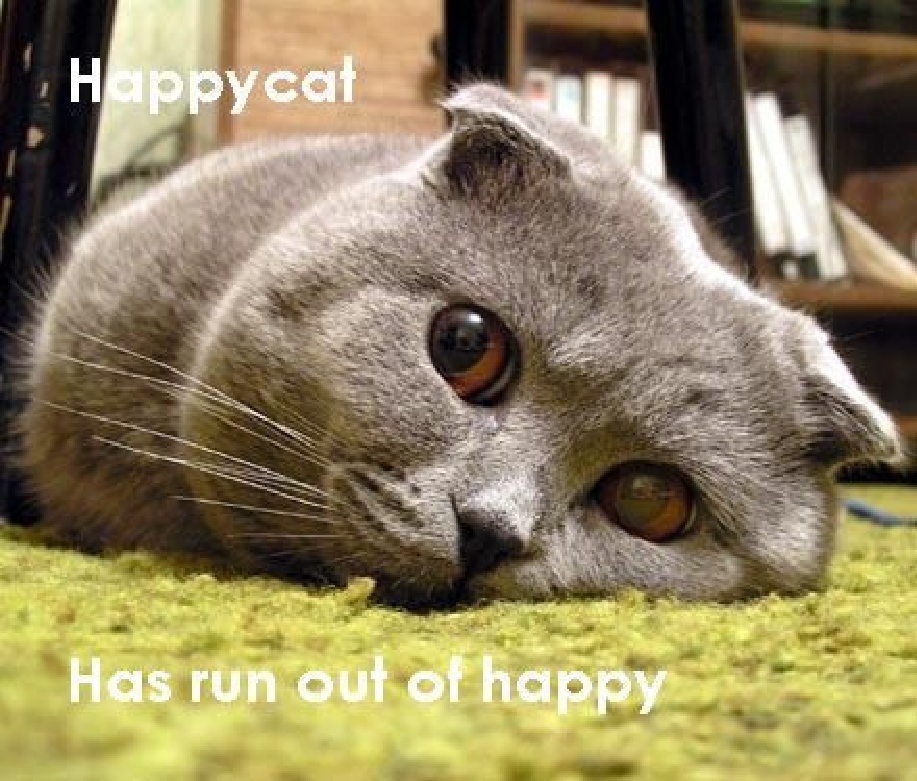
\includegraphics[width=3.25in, trim=1.25in 0.80in 0.90in 0.75in, clip]{figures/Main2_ProportionalToIndex_stdThread_shuffler}} \\
    \subfloat[omp dynamic]{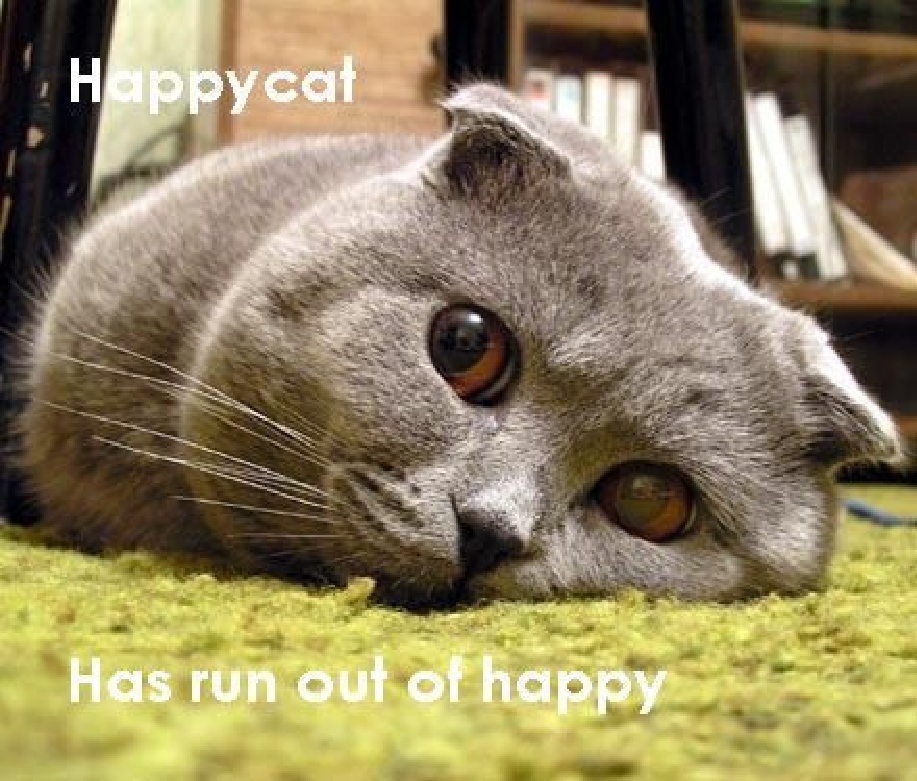
\includegraphics[width=3.25in, trim=1.25in 0.80in 0.90in 0.75in, clip]{figures/Main2_ProportionalToIndex_ompDynamic_shuffler}} & \\
    \subfloat[omp guided]{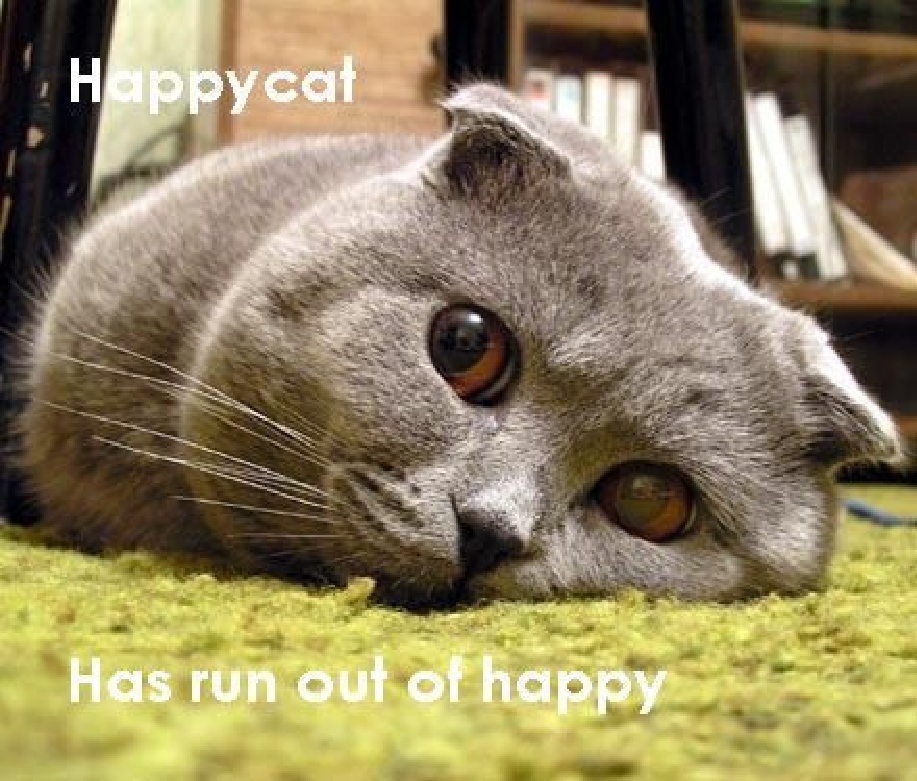
\includegraphics[width=3.25in, trim=1.25in 0.80in 0.90in 0.75in, clip]{figures/Main2_ProportionalToIndex_ompGuided_shuffler}} &
    \subfloat[tbb]{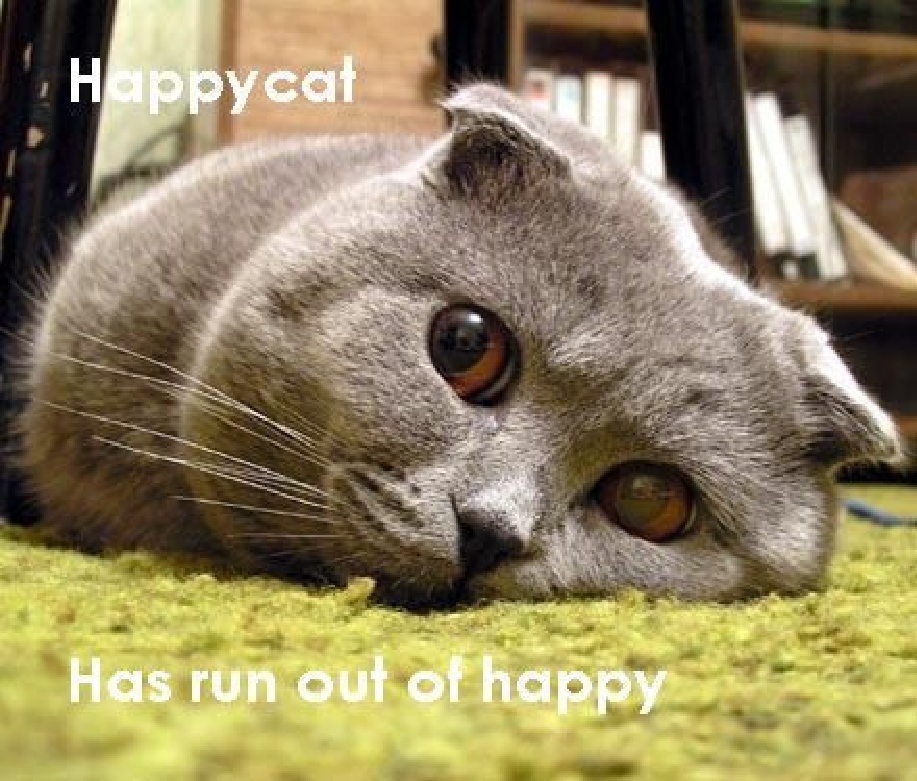
\includegraphics[width=3.25in, trim=1.25in 0.80in 0.90in 0.75in, clip]{figures/Main2_ProportionalToIndex_tbb_shuffler}} \\
    \end{tabular}
    \end{center}
    \caption{Performance for ProportionalToIndex polynomial order}
    \label{fig:Main2_proportionalToIndex}
  \end{figure}
}

{
  \begin{figure}[ht]
    \begin{center}
    \begin{tabular}{cc}
    \subfloat[Fixed Smallest Size]{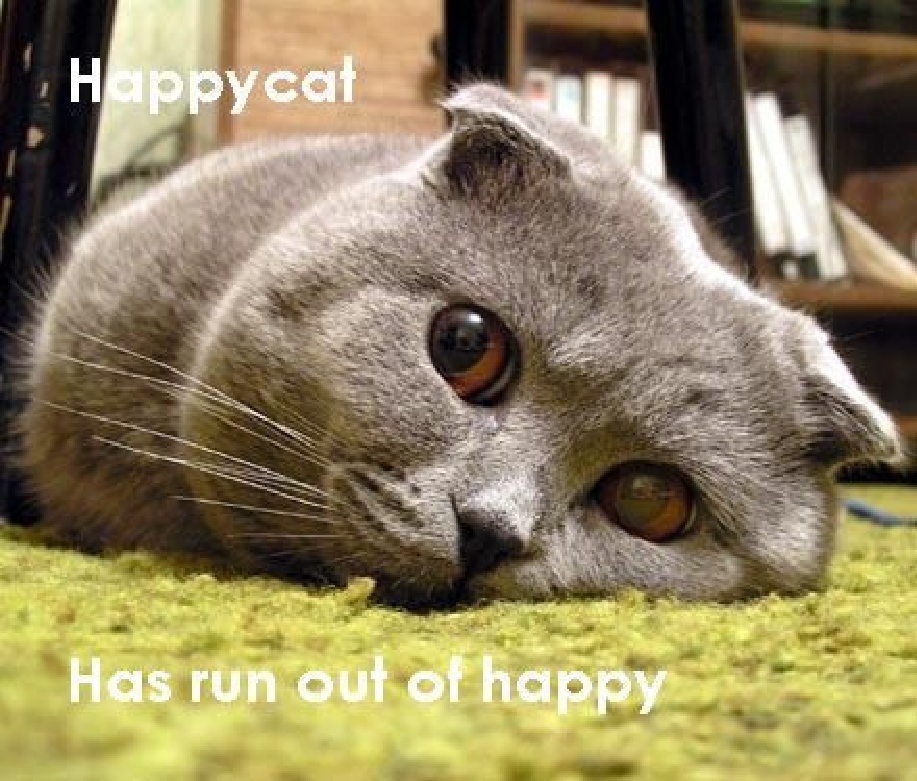
\includegraphics[width=3.0in]{figures/Main2_Fixed_2d_smallestSize_shuffler}} &
    \subfloat[ProportionalToIndex Smallest Size]{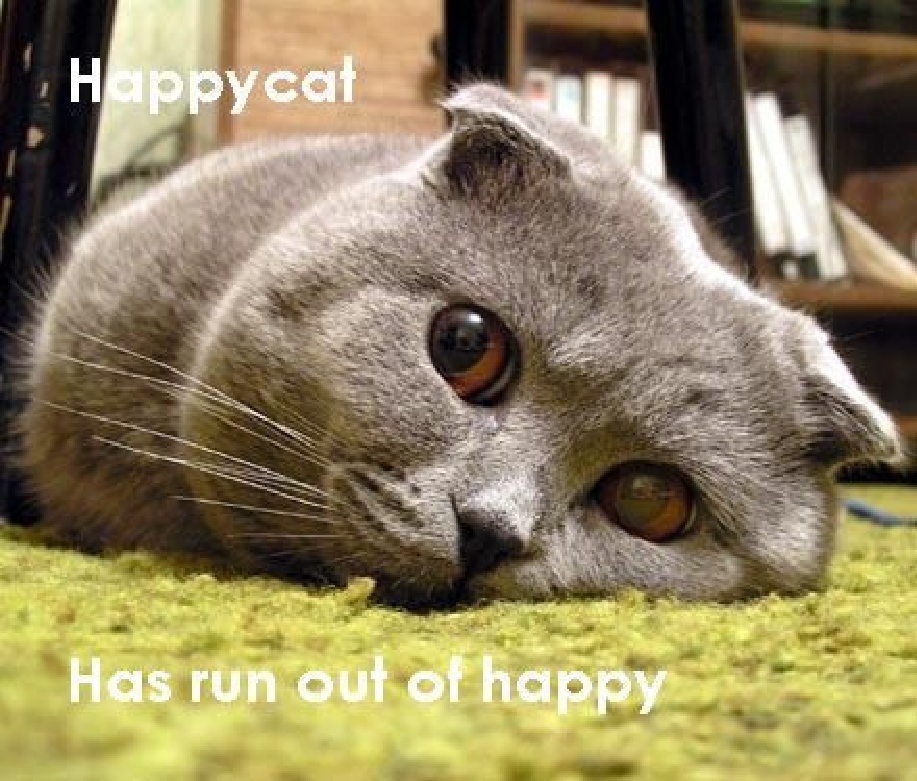
\includegraphics[width=3.0in]{figures/Main2_ProportionalToIndex_2d_smallestSize_shuffler}} \\
    \subfloat[Fixed Middle Size]{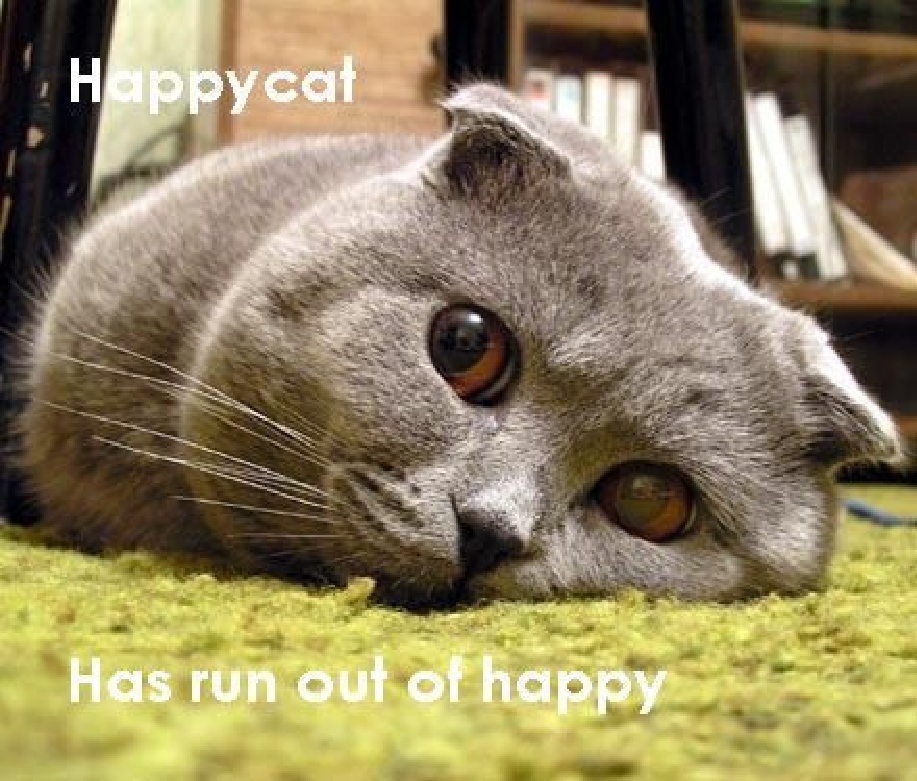
\includegraphics[width=3.0in]{figures/Main2_Fixed_2d_middleSize_shuffler}} &
    \subfloat[ProportionalToIndex Middle Size]{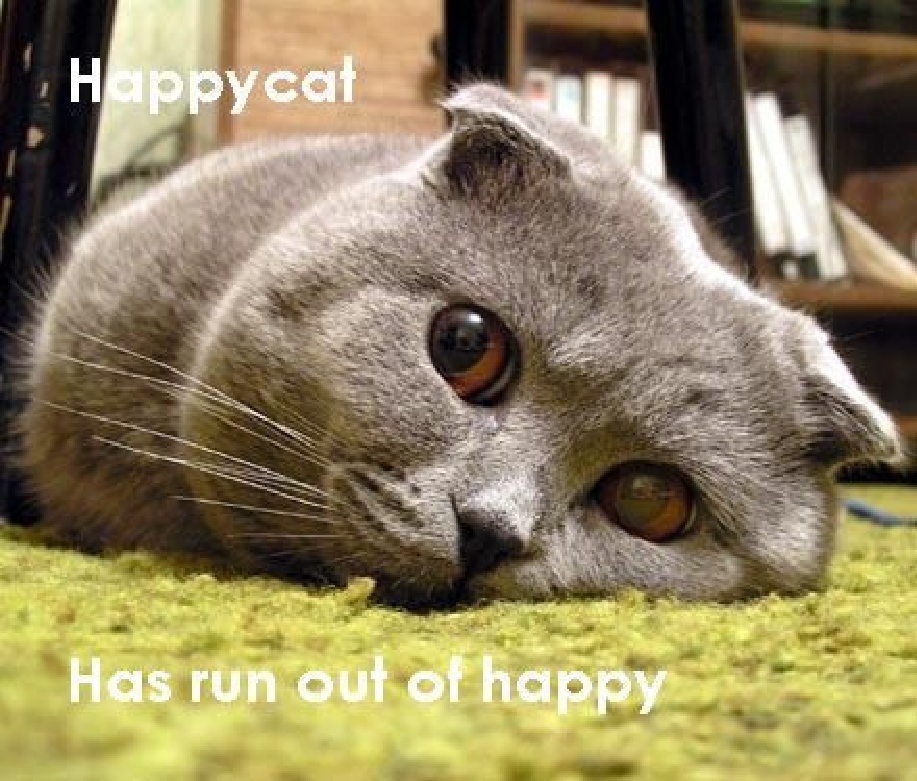
\includegraphics[width=3.0in]{figures/Main2_ProportionalToIndex_2d_middleSize_shuffler}} \\
    \subfloat[Fixed Largest Size]{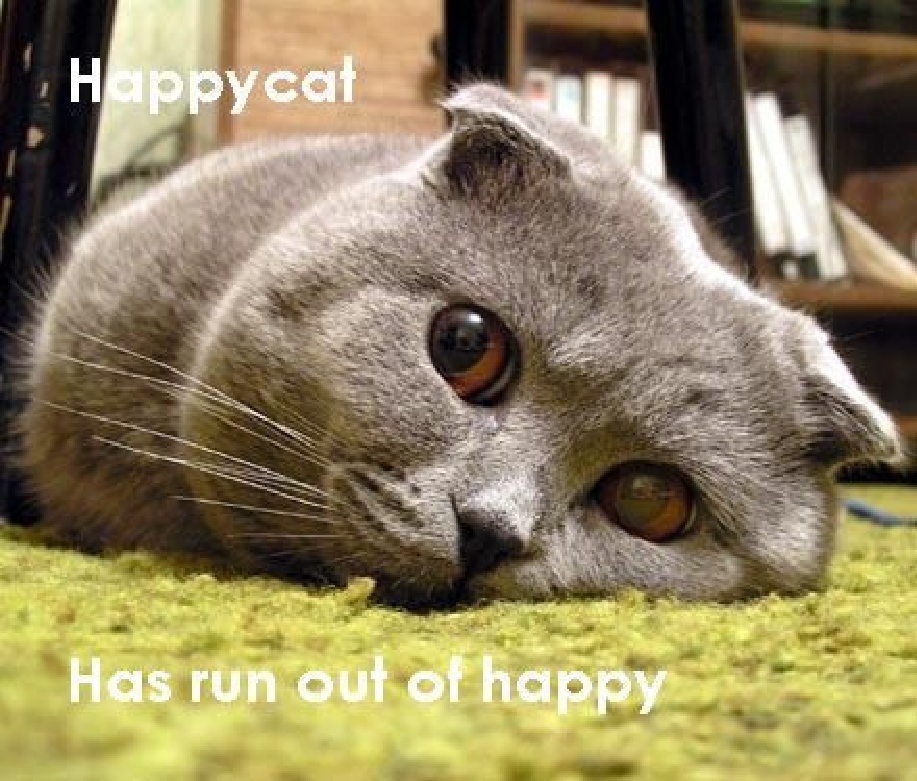
\includegraphics[width=3.0in]{figures/Main2_Fixed_2d_largestSize_shuffler}} &
    \subfloat[ProportionalToIndex Largest Size]{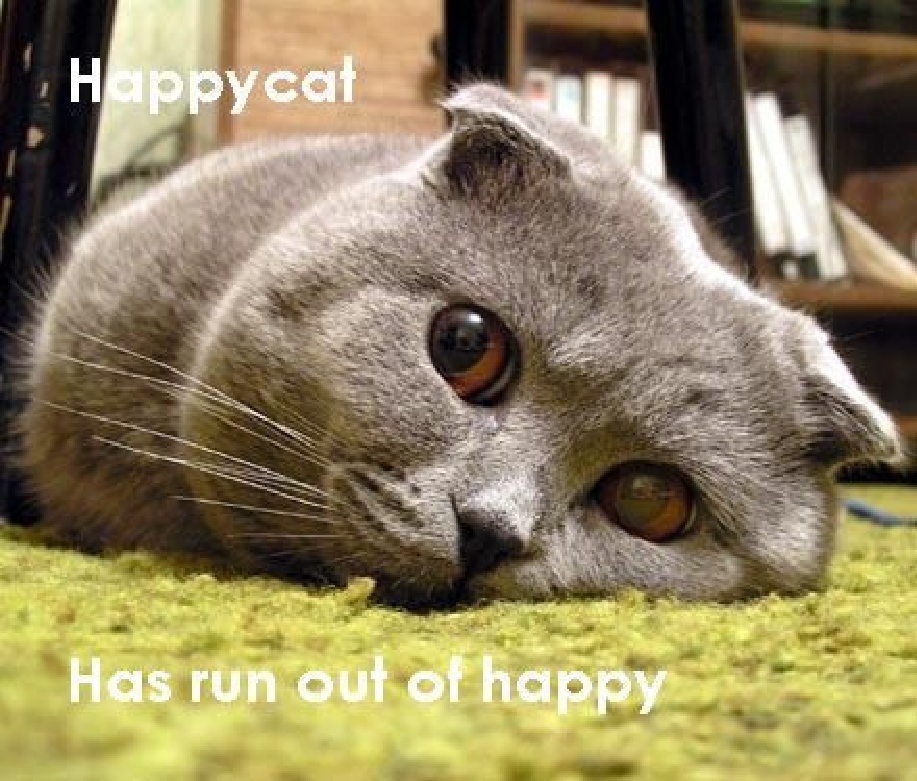
\includegraphics[width=3.0in]{figures/Main2_ProportionalToIndex_2d_largestSize_shuffler}} \\
    \end{tabular}
    \end{center}
    \caption{2d summaries for specific sizes}
    \label{fig:Main2_2dSummaries}
  \end{figure}
}

{
  \begin{figure}[ht]
    \begin{center}
    \begin{tabular}{cc}
    \subfloat[omp guided over tbb, Fixed]{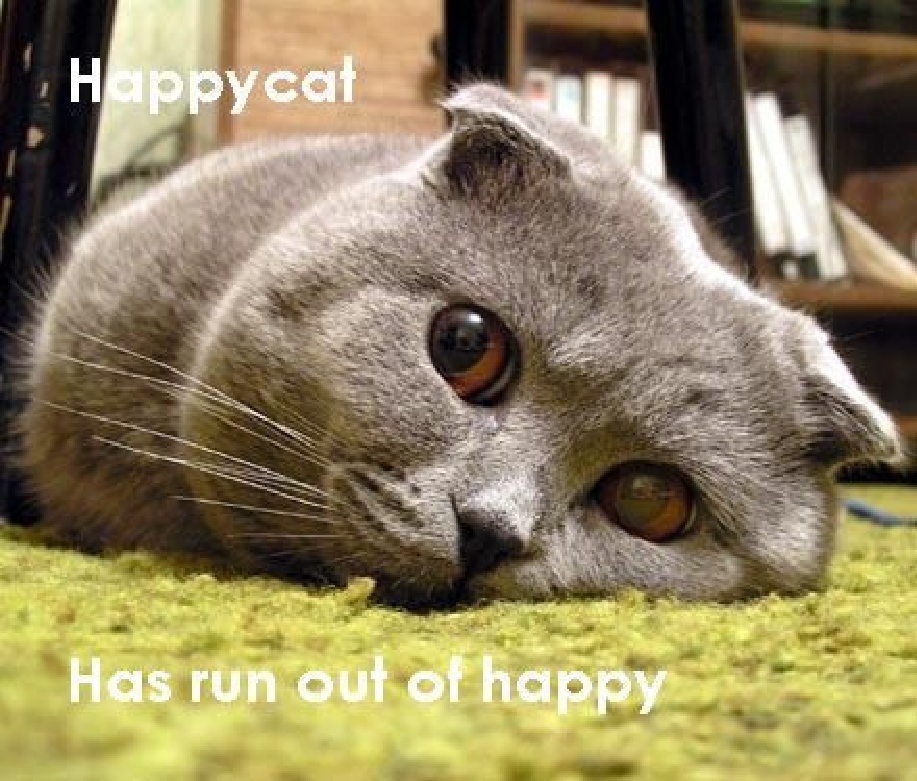
\includegraphics[width=3.25in, trim=1.25in 0.80in 0.90in 0.75in, clip]{figures/Main2_Fixed_ompGuidedVersusTbb_shuffler}} &
    \subfloat[tbb over omp guided, Fixed]{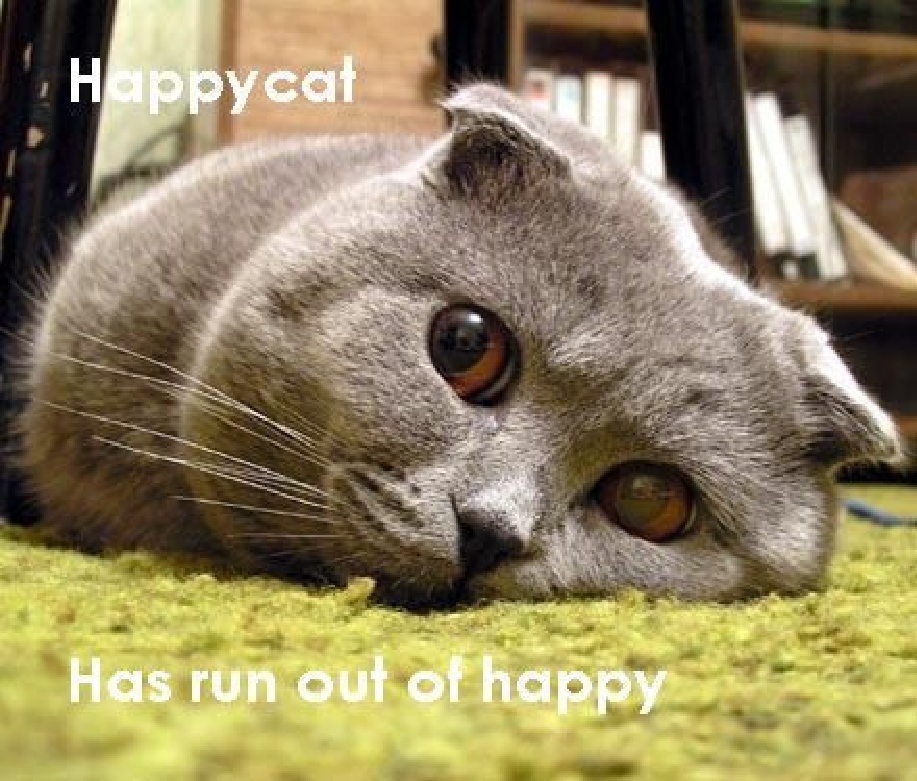
\includegraphics[width=3.25in, trim=1.25in 0.80in 0.90in 0.75in, clip]{figures/Main2_Fixed_tbbVersusOmpGuided_shuffler}} \\
    \subfloat[omp guided over tbb, ProportionalToIndex]{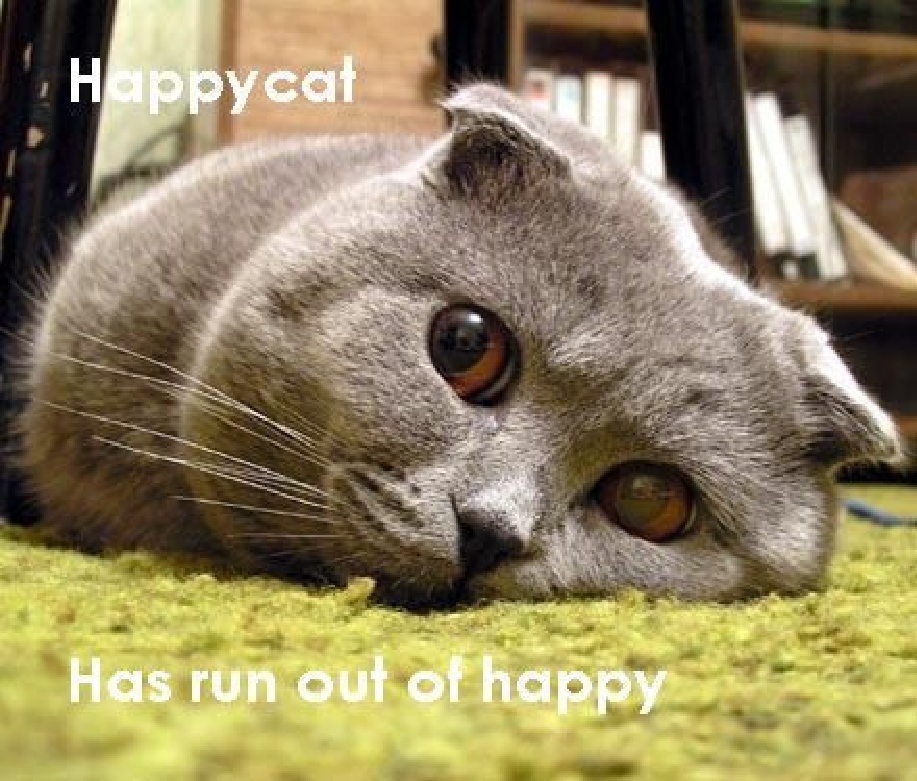
\includegraphics[width=3.25in, trim=1.25in 0.80in 0.90in 0.75in, clip]{figures/Main2_ProportionalToIndex_ompGuidedVersusTbb_shuffler}} &
    \subfloat[tbb over omp guided, ProportionalToIndex]{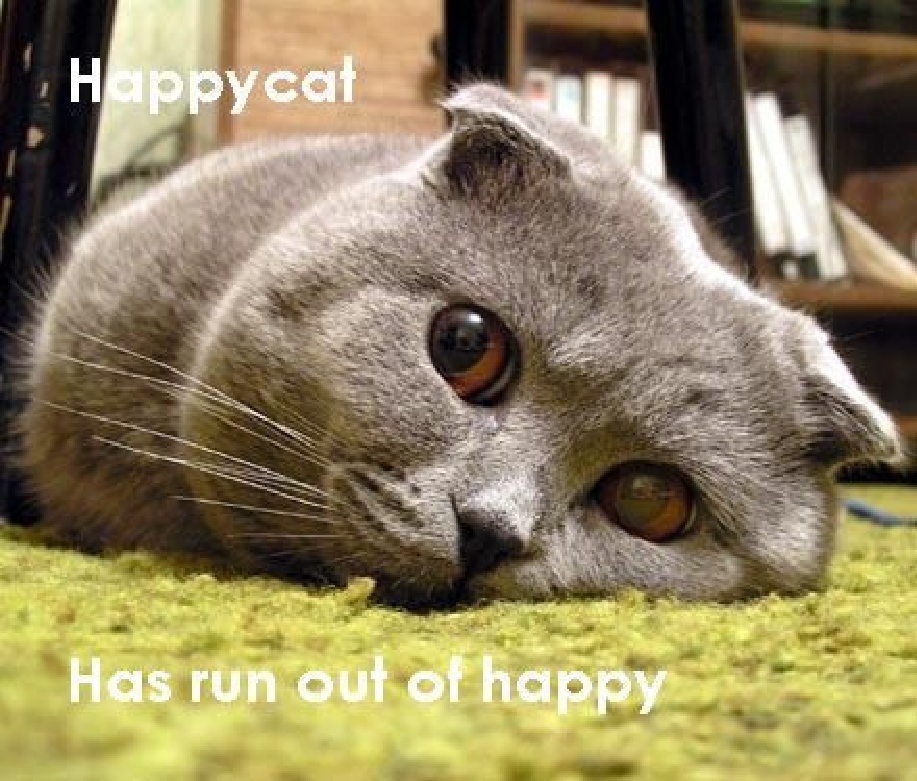
\includegraphics[width=3.25in, trim=1.25in 0.80in 0.90in 0.75in, clip]{figures/Main2_ProportionalToIndex_tbbVersusOmpGuided_shuffler}} \\
    \end{tabular}
    \end{center}
    \caption{Tbb versus omp guided for both scenarios}
    \label{fig:Main2_tbbVersusOmpGuided}
  \end{figure}
}

\fi

\FloatBarrier

\vfill











\eprob{50}{Locked, atomiced, and reduced: Histogram Calculations}

It is ludicrous to do something such as scalar integration with any threading method but reductions because the reductions are so cheap and the thread-private storage is so small.  
However, as described in class, there are situations in which you may not be able to use reductions (because they're expensive or the thread-private storage would be too large) and you will have to regulate access of threads to a common output location.  
In this problem, we'll examine performance for a situation in which you could do either reductions or regulated access.

We are going to calculate a histogram of the output values of some function for a bunch of inputs.  
Both the output and the input of the function are in the interval \texttt{[0, 1)}, and we'll calculate a histogram of the outputs for some number of buckets.

\begin{enumerate}[a)]
\item First, we'll make reduction, atomics, and lock versions without tbb.  You can use \texttt{openmp} or \texttt{std::thread}, but I recommend \texttt{openmp}.
  
\begin{enumerate}[1)]
  \item Implement the \textit{reduction} version of the histogram calculation in \texttt{calculateHistogram\_reduction}.  
  \item Implement the \textit{atomics} version of the histogram calculation in \texttt{calculateHistogram\_atomics}.  You can use either \texttt{pragma omp atomic} or the \texttt{std::atomic} type discussed \href{http://www.cplusplus.com/reference/atomic/atomic/}{here}.
  \item Implement the \textit{multiple lock} version of the histogram calculation in \texttt{calculateHistogram\_atomicFlagLocks}.  This function receives a \texttt{lockBucketSize}, which is the number of buckets each lock will be in charge of regulating.  For example, when \text{lockBucketSize} is 2, each lock is in charge of two buckets (so, you have lots of locks).  When \text{lockBucketSize} is 1024, each lock is in charge of 1024 buckets (so, you have few locks).
  
For practice, use a \href{http://en.cppreference.com/w/cpp/atomic/atomic_flag}{std::atomic\_flag} spinlock for your lock.  
If you have a \texttt{std::atomic\_flag lock}, you lock it with \texttt{while(lock.test\_and\_set(std::memory\_order\_acquire))} and release it with \\\texttt{lock.clear(std::memory\_order\_release)}.  An example is in the starter code.

\end{enumerate}

You don't need to say anything for this part of the problem, the plot will come later.

\item Now, we'll make reduction, atomics, and lock versions with tbb.

\begin{enumerate}[1)]
  \item Implement a \textit{tbb reduction} version of the histogram calculation in \texttt{calculateHistogram\_tbbReduction}.  
  \item Implement a \textit{tbb atomics} version of the histogram calculation in \texttt{calculateHistogram\_tbbAtomics}.  
Use a \href{http://www.threadingbuildingblocks.org/docs/help/reference/synchronization/atomic\_cls.htm}{tbb::atomic} type described \href{http://www.threadingbuildingblocks.org/docs/help/tbb_userguide/Atomic\_Operations.htm}{here}, \textit{not} \texttt{std::atomic}.
  \item Implement a \textit{tbb multiple lock} version of the histogram calculation in \texttt{calculateHistogram\_tbbLocks}.  
Threading Building Blocks provides several mutexes described \href{https://www.threadingbuildingblocks.org/docs/help/tbb_userguide/Mutex_Flavors.htm}{here}; use a \texttt{tbb::speculative\_spin\_mutex} for the lock.
A neat way of using \texttt{tbb} locks is to use their \texttt{scoped\_lock} version, which enables some interesting usage patterns.
You make a \texttt{scoped\_lock} when you want to grab a lock, and you let it fall out of scope when you want to free the lock.

\begin{verbatim}
tbb::speculative_spin_mutex lock;
{
  tbb::speculative_spin_mutex::scoped_lock scopedLock(lock);
  // protected stuff
  // lock is released when scopedLock goes out of scope on the next line
}
\end{verbatim}

\end{enumerate}

You don't need to say anything for this part of the problem, the plot will come later.

\item The provided rendering script makes 3d plots of the speedup of the two \textit{multiple lock} versions versus \texttt{numberOfThreads} and \texttt{lockBucketSize}.  Comment on these results.

\ifSolutions
\textbf{Solution:}

{
  \begin{figure}[ht]
    \begin{center}
    \begin{tabular}{c}
    \subfloat[non-tbb locks]{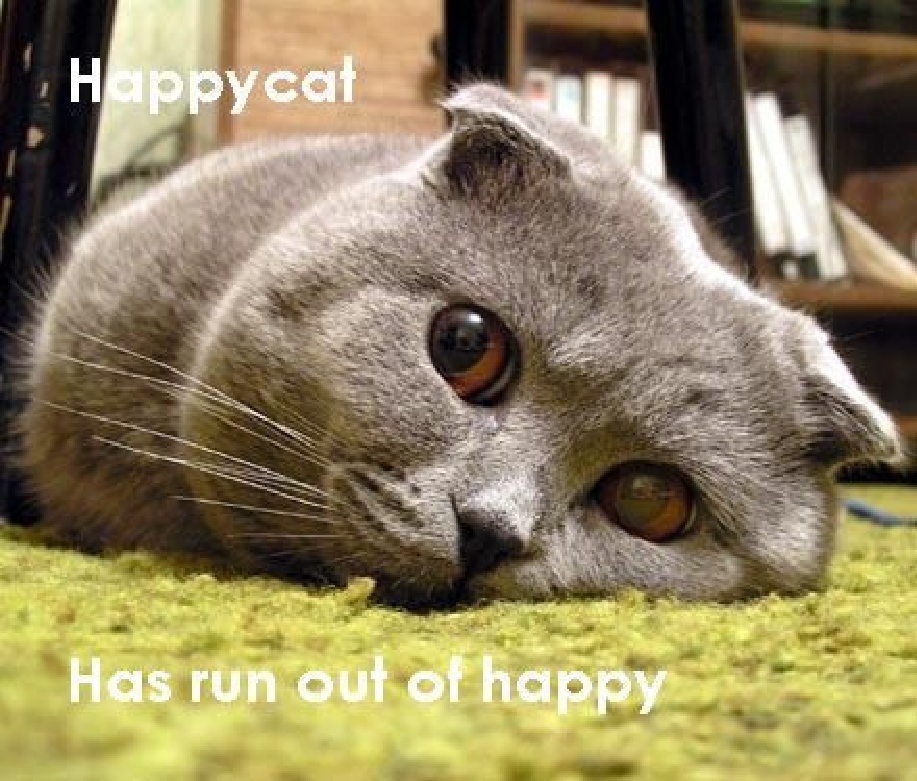
\includegraphics[width=4.0in, trim=1.75in .6in .9in 0.60in, clip]{figures/Main3_atomicFlagLocks_shuffler}} \\
    \subfloat[tbb locks]{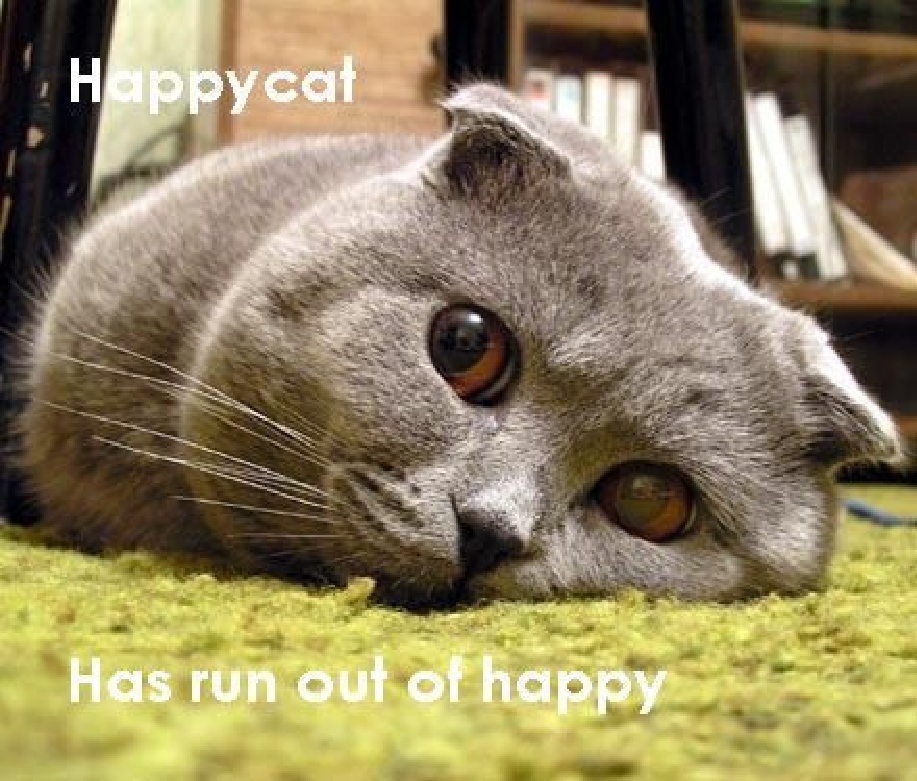
\includegraphics[width=4.0in, trim=1.75in .6in .9in 0.60in, clip]{figures/Main3_tbbLocks_shuffler}} \\
    \end{tabular}
    \end{center}
    \caption{Performance of locking methods for the histogram}
    \label{fig:Main3_locking}
  \end{figure}
}

\fi

\item The provided rendering script makes a 2d plot of the four lock-free methods (reduction and atomics versions) as well as the two (tbb and non-tbb) locked methods (using their respective optimal \texttt{lockBucketSizes}).  Comment on these results.

Note: you will need to update which ``slice'' to use in the locked versions to whichever slice does the best.  
To plot one ``slice'' of the times from one of the locked versions, you can pick the desired slice out of the \texttt{tbbLocksTimes} object with slicing by column: \texttt{tbbLocksTimes[:,0]} is the first column, \texttt{tbbLocksTimes[:,4]} is the fifth column, etc.
As of now, the columns correspond to the \texttt{lockBucketSizes} in the following way: \texttt{[1, 2, 4, 8, 16, 32, 64]}.

\ifSolutions
\textbf{Solution:}

{
  \begin{center}
  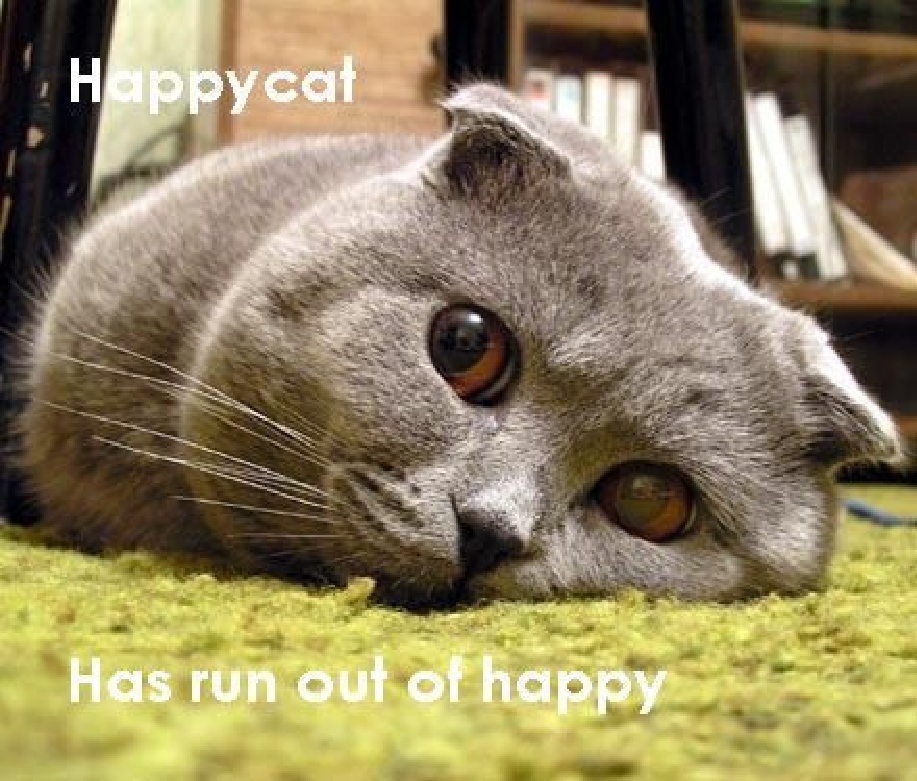
\includegraphics[width=6.0in]{figures/Main3_summary_shuffler}
  \end{center}
}

\fi

\end{enumerate}

\FloatBarrier

\vfill








\eprob{15}{Back to the Real World}

Provide short (but sufficient) answers to the following prompts:

\begin{enumerate}[a)]

\item Without using the word ``factory'', explain as you would to a ``non-technical'' friend of yours the difference between \texttt{tbb} and other threading systems.

\ifSolutions
\textbf{Solution:}

\fi

\item Explain as you would to a ``non-technical'' friend of yours the difference between and when you would use \texttt{tbb's} \texttt{parallel\_reduce} versus \texttt{parallel\_for}.

\ifSolutions
\textbf{Solution:}

\fi

\item Suppose your lab-mate says to you ``oh, threading is easy.  You just throw \texttt{pragma omp parallel for} in some places.''  
How would you respond?

\ifSolutions
\textbf{Solution:}

\fi

\item Using multiple threads does not always improve performance.  
Describe a program for which threading would not improve performance but you'd get essentially the same speed as without threads.  
Describe another situation in which you get worse performance by using multiple threads.

\ifSolutions
\textbf{Solution:}

\fi

\end{enumerate}

\eprob{5}{Feedback}

\begin{enumerate}[a)]
\item How much total time did you spend on this assignment?
\item Of the total time, how much total time did you spend ``flailing'' on little annoying things that are not the main point of the assignment?
\item Did you have any ``aha'' moments where something clicked?  If so, on what problems or parts?
\item Can you give me any feedback on this assignment?
\end{enumerate}

\vfill

\vskip 1cm
\total

\end{document}

todo: finish the fortran webserver problem for homework 9.
